Проводится исследование из области солнечной энергетики. На рис. 1 показана схема установки для исследования фотоэлектрических характеристик.

\begin{figure}[H]
	\begin{center}
		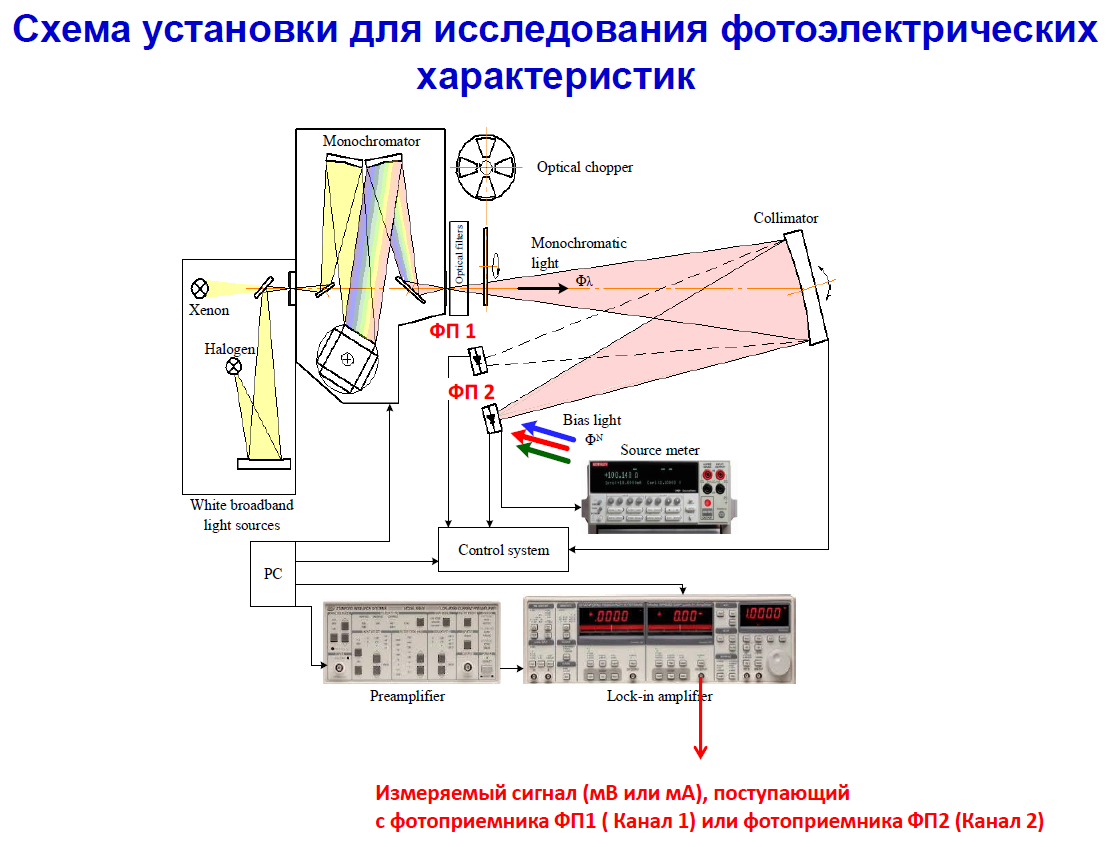
\includegraphics[scale=0.8]{problem1}
		\label{pic:problem1}
		\caption{Схема установки для исследования фотоэлектрических характеристик}
	\end{center}
\end{figure}

Калибровка датчика ФП2 производится по эталону ФП1. Зависимость между квантовыми эффективностями датчиков предполагается постоянной для каждой пары наборов измерений:

\begin{equation}
	QE_2 = \frac{I_2}{I_1} \cdot QE_1
\end{equation}

где $QE_2$, $QE_1$ -- эталонная эффективность эталонного и исследуемого датчика, $I_2$, $I_1$ -- измеренные токи. Данные с датчиков находятся в файлах \textbf{Канал2\_800nm\_0.2.csv}, \textbf{Канал1\_800nm\_0.2.csv} и полагаются линейными.

Требуется определить коэффициент калибровки:

\begin{equation}
R_{21} = \frac{I_2}{I_1}
\end{equation}

на основе линейной регрессии на множестве интервальных данных и коэффициента Жаккара.